\chapter{Acoustic Diffraction}
%************************************************
\begin{flushright}
August 26 and 27, 2013 \\
% [$3 \times 6 hours spent$]
\end{flushright}

\section{Theory}
	Certain assumptions made in the following discussion have been explicitly stated here for clarity.
	\begin{enumerate}
		\item The diffraction grating formed has almost zero thickness
		\item A diffraction pattern is observed only when a standing wave is produced
		\item Snell's law can be ignored in the consideration of the diffraction pattern
	\end{enumerate}
	The idea of the experiment is to estimate the speed of sound in distilled water, by producing an acoustic diffraction grating. The setup is as shown in \autoref{e2_setup}.

	\begin{figure}[bth]
		\begin{center}
			
\includegraphics[width=1.3\linewidth]{gfx/e2_acousticGrating}
		\end{center}
		\caption[Setup for Acoustic Diffraction]{Setup for Acoustic Diffraction}
	\label{e2_setup}
	\end{figure}

	Debye and Sears, in 1932 demonstrated that light diffracts while it passes through a liquid medium excited to ultrasonic vibrations. They explained it by saying that the density maxima and minima of the standing wave obtained in the liquid behaved like an optical diffraction grating, where the grating constant was the wavelength of this ultrasonic wave. Therefore, this method can be used to determine the speed of sound in the medium once we have determined the wavelength of sound by measuring the distance between the ultrasonic source and the diffraction image.

	The generation of standing wave in a medium causes changes in density due to pressure nodes and anti-nodes of the sound wave. These density fluctuations in turn cause variations in refractive index which diffracts a beam of light travelling perpendicular to the direction of sound as if it had been diffracted from a diffraction grating of spacing $2d=\lambda_\text{sound}$ for a standing wave. The sound field is set up by driving a piezoelectric crystal at a given frequency.

	The setup consists of a laser, an ultrasonic probe i.e. a piezoelectric crystal, a cuvette filled with a medium (in this case, distilled water), a screen and a frequency generator. The known result $d \sin \theta = n \lambda$ is used for finding $d$ and therefore $\lambda_\text{sound}$, where small angle approximation is used to write 
	\begin{equation*}0
		\sin \theta = \frac {\text{in the plane of the screen, displacement from the centre}}{\text{distance of the grating from the screen}}
	\end{equation*}

	\textsc{bragg's diffraction}
	An electromagnetic radiation which reflects from the surface of a substance has travelled less distance than the one which reflects from a plane of atoms inside the crystal. The penetrating electromagnetic radiation travels down to the internal layer, reflects, and travels back over the same distance before being back at the surface. The distance travelled depends on the separation of the layers and the angle at which the electromagnetic radiation entered the material. For this wave to be in phase with the wave which reflected from the surface it needs to have travelled a whole number of wavelengths while inside the material. Bragg expressed this in an equation now known as Bragg's Law, mathematically stated as 
	\begin{equation*}
	n \lambda = 2d \sin \theta
	\end{equation*}
	where $\lambda$ is the wavelength of the incident radiation, $d$ is the spacing between the scattering planes and $\theta$ the angle between them.
	It gives the angles at which the radiation, reflected off the scattering plane interferes constructively and produces a peak (a Bragg peak).
	First proposed by William Lawrence Bragg and William Henry Bragg in 1912, it is used as a tool to study crystals in the form of X-ray and neutron diffraction. 





\section{Further Questions}
	\begin{itemize}
		\item Study braggs diffraction and raman diffraction from Photonics by Teichi 
		\item How does the dimension of the medium affect the pattern?
		\item Can we realize Braggs diffraction in this experiment?
		\item Will the diffraction pattern change upon movement of the diffraction grating? Diffraction pattern formation in case no standing waves are formed?
		\item If the diffraction grating is infinite , will its movement affect the diffraction pattern --- it will be phase shifted
	\end{itemize}

\section{Calculations and Results}
	The observations have been listed in \autoref{e2_obs}. The results have been listed in \autoref{e2_result}. \autoref{e2_graph} is the graph obtained.
	\par
	The speed of sound was found out to be 1312 $m/s$ and 1250 $m/s$ using either sides of the graph.

	\begin{figure}[bth]
		\begin{center}
			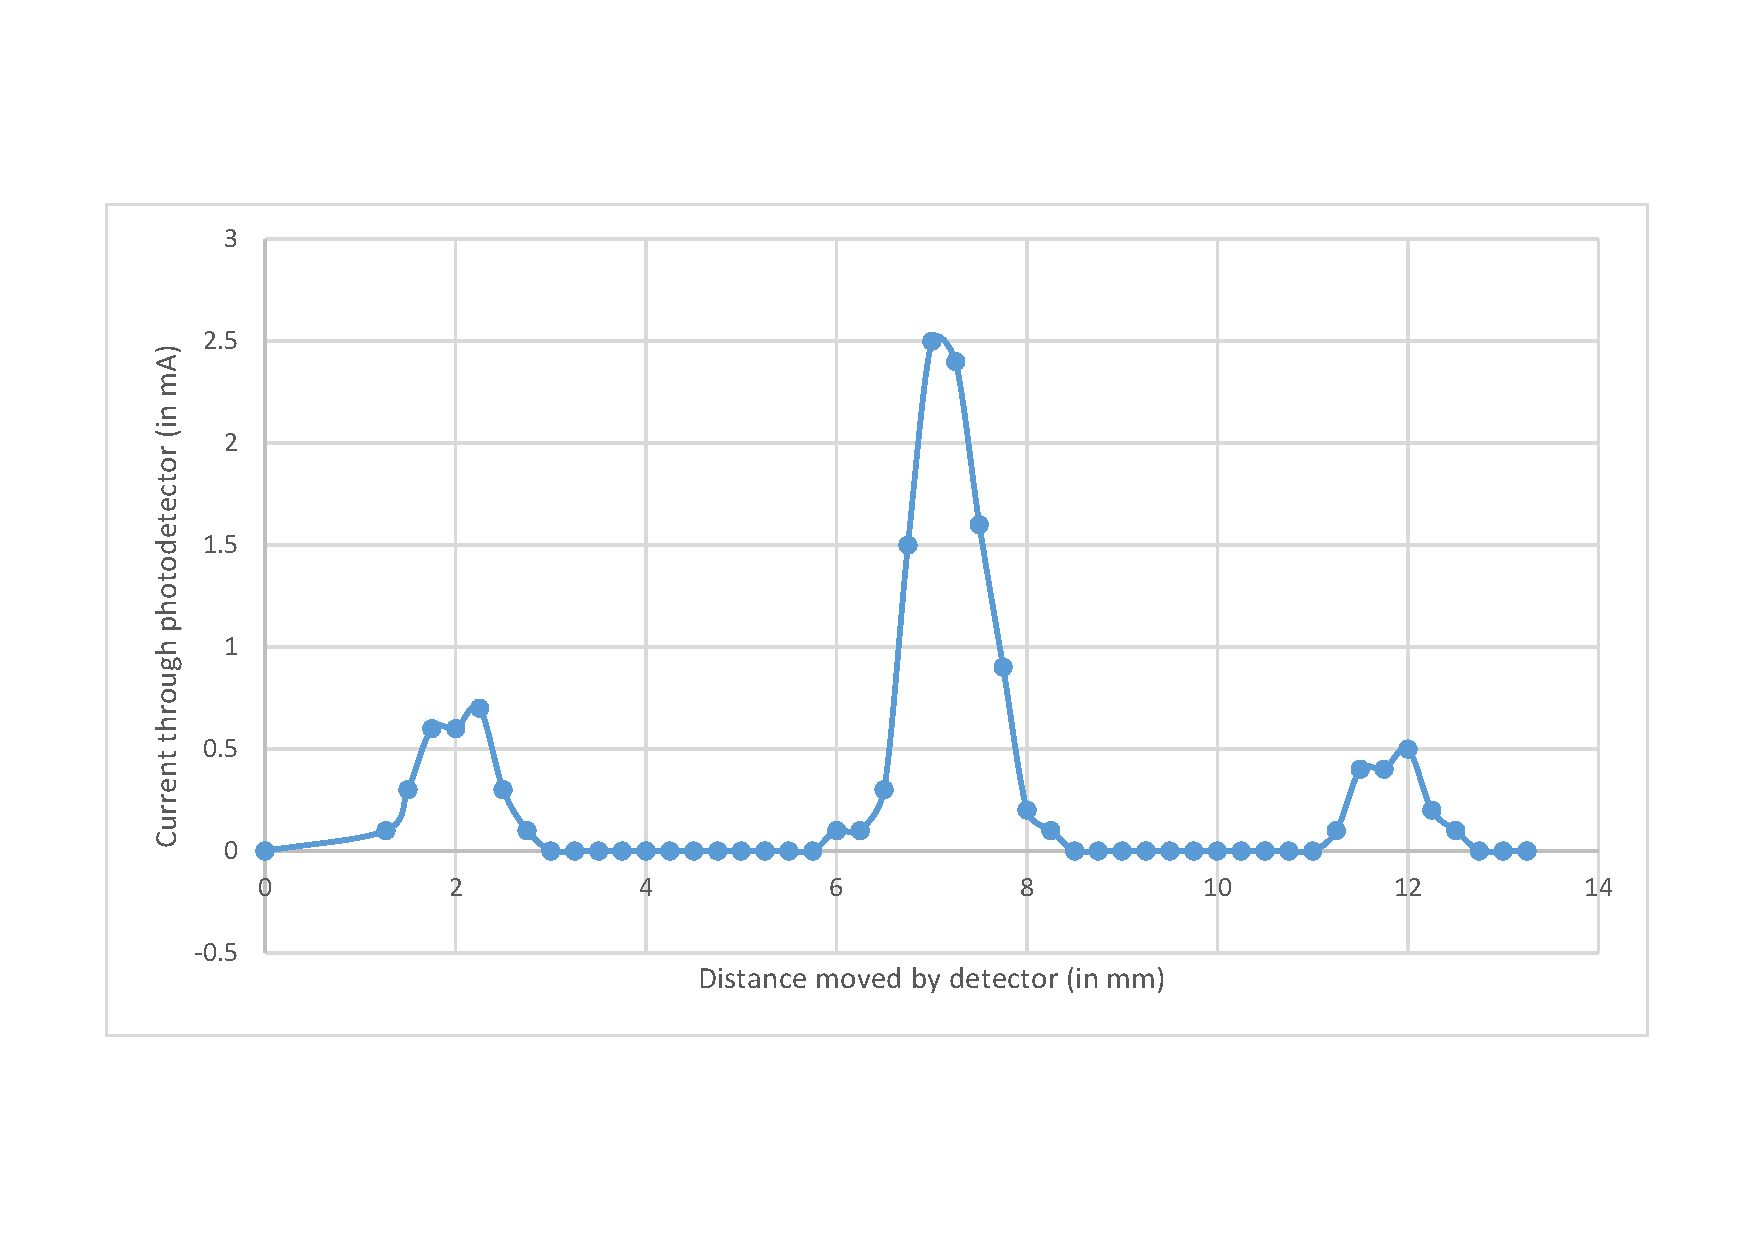
\includegraphics[width=1.3\linewidth]{gfx/e2_graph}
		\end{center}
		\caption[Graph]{Graph for Acoustic Diffraction}
	\label{e2_graph}

	\end{figure}
	\begin{figure}[bth]
		\begin{center}
			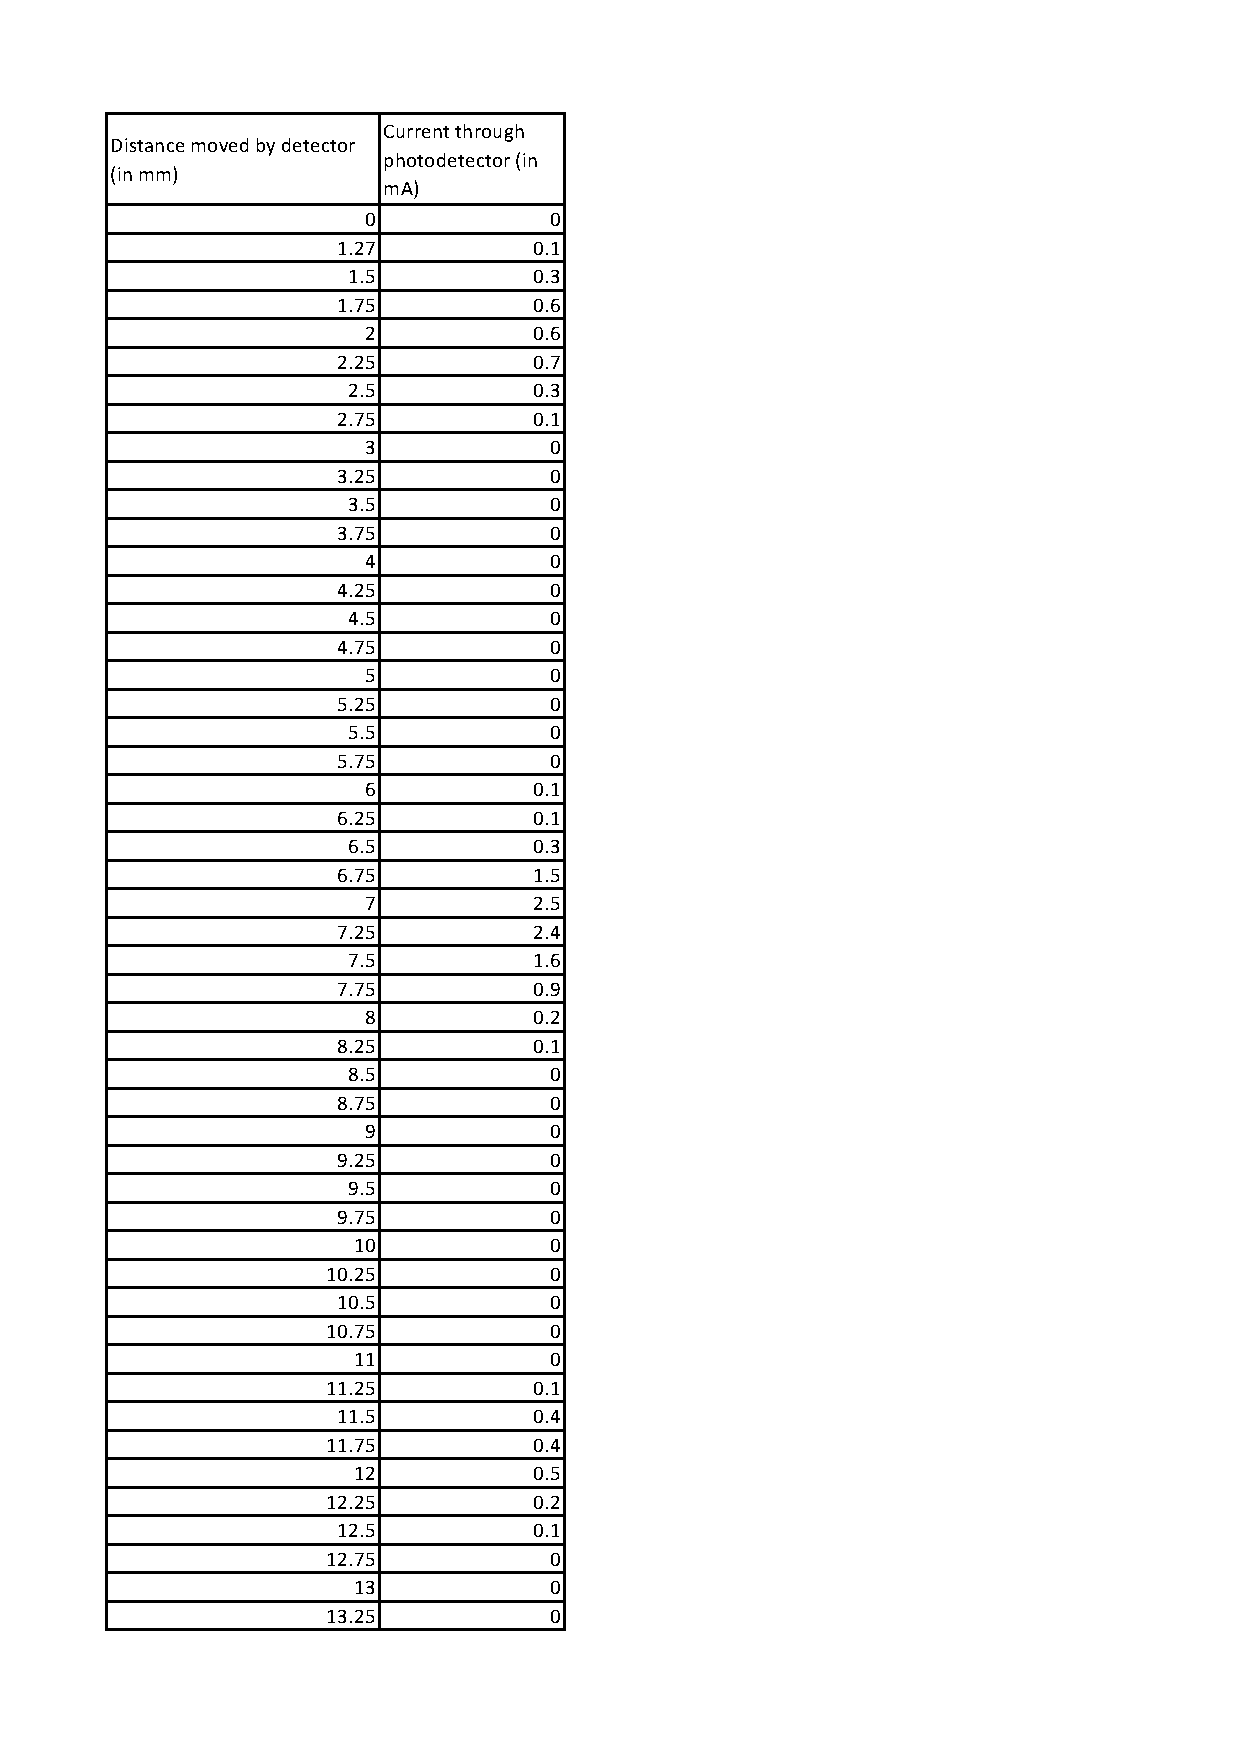
\includegraphics[width=1.3\linewidth]{gfx/e2_obs}
		\end{center}
		\caption[Observations]{Observations for Acoustic Diffraction}
	\label{e2_obs}
	\end{figure}

	\begin{figure}[bth]
		\begin{center}
			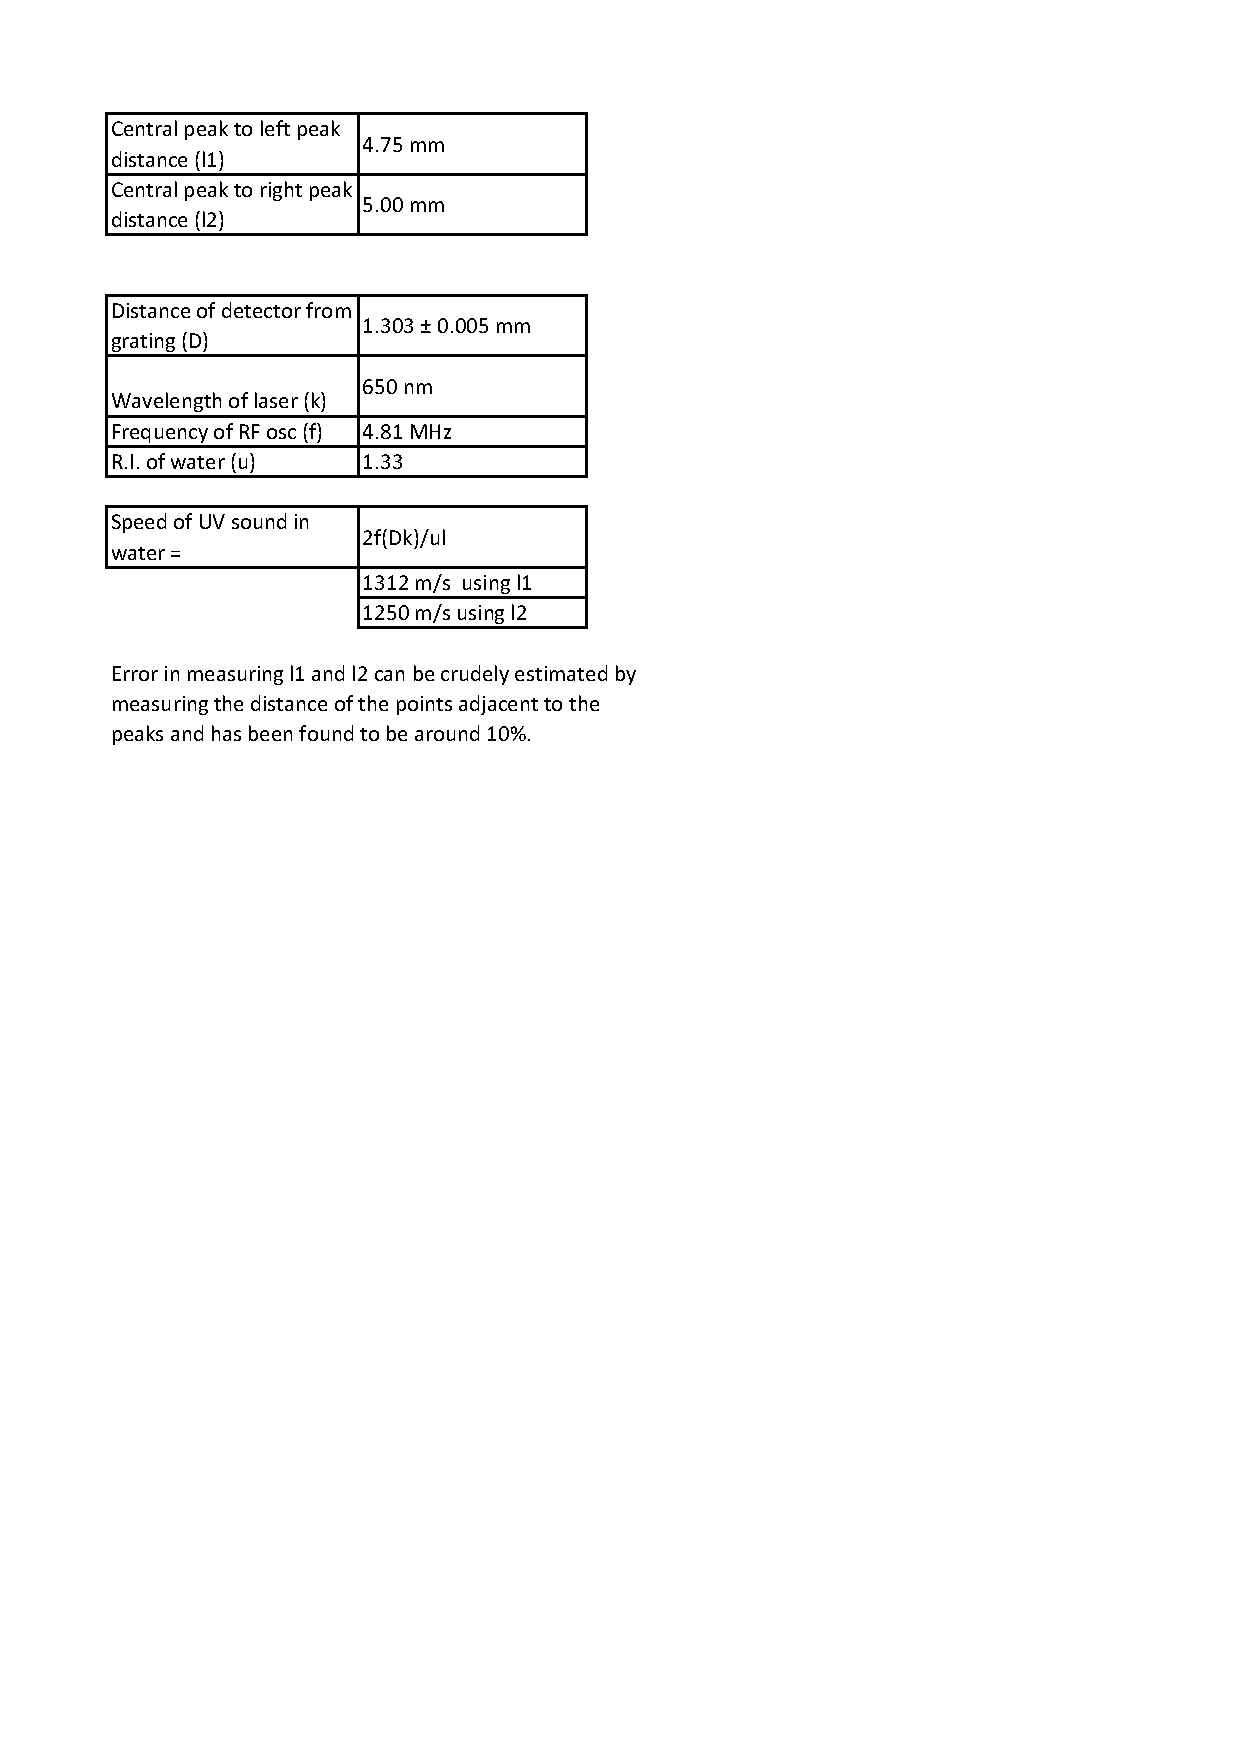
\includegraphics[width=1.3\linewidth]{gfx/e2_results}
		\end{center}
		\caption[Calculations and Results]{Results and Calculations for Acoustic Diffraction}
	\label{e2_result}
	\end{figure}

